% !TEX program = xelatex
% 中国商品期货机器学习因子投资：10分钟课程答辩
% Theme: #013E75 / #A42423 / #FFFBF0
\documentclass[aspectratio=169,10pt]{beamer}
\usepackage{academicminimal}
\usepackage{threeparttable}
\graphicspath{{report_assets/}{report_figures/}}
\AtBeginSection[]{} % 本汇报不插入额外章节页，以控制在36页

\title{机器学习能否改善\\中国商品期货因子投资？}
\subtitle{统一数据、标签、样本外检验与交易成本下的证据}
\author{主题七项目组}
\institute{课程项目答辩}
\date{2026年7月}

% 固定总页数，避免附录模式改变 Beamer 的自动分母。
\renewcommand{\inserttotalframenumber}{39}

\newcommand{\tagbox}[1]{\tikz[baseline=(X.base)]\node[fill=AcademicBlueSoft,draw=AcademicLine,rounded corners=1.5pt,inner xsep=4pt,inner ysep=2pt,font=\tiny,text=AcademicNavy](X){#1};}
\newcommand{\redtag}[1]{\tikz[baseline=(X.base)]\node[fill=AcademicRedSoft,draw=AcademicRed!35,rounded corners=1.5pt,inner xsep=4pt,inner ysep=2pt,font=\tiny,text=AcademicRed](X){#1};}
\newcommand{\resultbar}[4]{%
  \begin{tikzpicture}[baseline]
    \node[anchor=east,font=\scriptsize] at (0,0) {#1};
    \fill[AcademicLine!55] (0.15,-0.10) rectangle (4.6,0.10);
    \ifdim #2pt>0pt
      \fill[#3] (2.375,-0.10) rectangle ({2.375+#2},0.10);
    \else
      \fill[#3] ({2.375+#2},-0.10) rectangle (2.375,0.10);
    \fi
    \draw[AcademicMuted,line width=.35pt] (2.375,-0.16)--(2.375,0.16);
    \node[anchor=west,font=\scriptsize\bfseries,text=#3] at (4.72,0) {#4};
  \end{tikzpicture}}

\begin{document}

% ==================== MAIN TALK: 24 slides / 600 seconds ====================

% 01 — 15s
\begin{frame}[plain]
  \titlepage
  \begin{tikzpicture}[remember picture,overlay]
    \node[anchor=south west,text=AcademicIvory!86,font=\small] at ([xshift=10mm,yshift=13mm]current page.south west)
      {30个品种\quad $\cdot$\quad 2015--2025\quad $\cdot$\quad 2019--2025 OOS\quad $\cdot$\quad 5bps};
  \end{tikzpicture}
\end{frame}

% 02 — 25s
\begin{frame}{团队分工与部分成员荣誉}
  \vspace{-1mm}
  \begin{columns}[T,onlytextwidth]
    \begin{column}{0.66\textwidth}
      {\scriptsize\bfseries\color{AcademicNavy}跨校协作分工}\par
      \vspace{0.7mm}
      \renewcommand{\arraystretch}{1.08}
      \setlength{\tabcolsep}{2.2pt}
      \begin{tabularx}{\linewidth}{@{}p{1.75cm}p{1.05cm}p{2.45cm}X@{}}
        \toprule
        \tiny\bfseries 学校·专业 & \tiny\bfseries 成员 & \tiny\bfseries 分工 & \tiny\bfseries 主要职责 \\
        \midrule
        \tiny 湖南财政经济学院·金融科技 & \tiny 刘坤 & \tiny 底层数据工程与整合 & \tiny 下载、清洗、对齐并预处理全市场量价、现货、仓单与库存等异构数据。 \\
        \tiny 上海交通大学·统计学 & \tiny 王晨宇 & \tiny 基础因子挖掘与策略探索 & \tiny 梳理商品市场逻辑，构建、筛选基础Alpha因子并开展初步有效性检验。 \\
        \tiny 复旦大学·数学 & \tiny 沈君阳 & \tiny 传统线性基准与多因子建模 & \tiny 构建等权多因子、单因子分层排序与多元线性回归，确立传统统计Baseline。 \\
        \tiny 上海交通大学·海洋--金融 & \tiny 郝铭梁 & \tiny 树模型与集成学习比较 & \tiny 构建正则化LightGBM、XGBoost与随机森林，并与传统方法横向评估。 \\
        \tiny 复旦大学·统计学 & \tiny 吴易航 & \tiny 前沿图神经网络探索 & \tiny 探索GNN在商品期货产业链中的应用，开展图结构横向特征提取实验。 \\
        \tiny 复旦大学·药学--AI双学位 & \tiny 刘梵佑 & \tiny 深度机器学习、统筹与交付 & \tiny 设计CNN--Transformer双头网络，开展抗过拟合与回撤验证；统筹模型比较并主导报告及答辩交付。 \\
        \bottomrule
      \end{tabularx}
    \end{column}
    \begin{column}{0.31\textwidth}
      {\scriptsize\bfseries\color{AcademicRed}部分团队成员 / 项目荣誉}\par
      \vspace{0.8mm}
      \begin{tikzpicture}[
        award/.style={draw=AcademicLine,fill=AcademicWhite,rounded corners=1.5pt,text width=36mm,inner xsep=2.2mm,inner ysep=1.3mm,align=left,font=\fontsize{5.3}{6.2}\selectfont},
        node distance=1.25mm
      ]
        \node[award] (a1) {第十五届“挑战杯”中国大学生创业计划竞赛\\\textcolor{AcademicRed}{上海市特等奖}};
        \node[award,below=of a1] (a2) {2026 MCM美国大学生数学建模竞赛\\\textcolor{AcademicRed}{F奖}};
        \node[award,below=of a2] (a3) {第八届“搜知杯”全国财经高校信息素养大赛\\\textcolor{AcademicRed}{全国一等奖}};
        \node[award,below=of a3] (a4) {第八届“中青杯”全国大学生数学建模竞赛\\\textcolor{AcademicRed}{全国二等奖}};
        \node[award,below=of a4] (a5) {第十六届“iCAN杯”大学生创新创业大赛\\\textcolor{AcademicRed}{全国三等奖}};
        \node[award,below=of a5] (a6) {第九届全国高校经济决策虚仿实验大赛智慧银行数字化运营竞赛\\\textcolor{AcademicRed}{全国三等奖、区域赛一等奖}};
        \node[award,below=of a6] (a7) {第十六届Mathor Cup高校数学建模/应用挑战赛\\\textcolor{AcademicRed}{区域赛二等奖}};
      \end{tikzpicture}
    \end{column}
  \end{columns}
\end{frame}

% 03 — 20s
\begin{frame}{先给答案：改善预测，不保证改善净收益}
  \begin{center}
    \metric{0.0065}{典型单因子Rank IC中位数}
    \hfill
    \metric{0.0247}{Ridge Rank IC}
    \hfill
    \metric{0.454}{HCGNN 5bps Sharpe}
  \end{center}
  \vspace{1mm}
  \begin{columns}[T,onlytextwidth]
    \begin{column}{0.48\textwidth}
      \begin{block}{预测层}
        学习型模型能够整合分散弱信号，Ridge的横截面排序能力明显高于典型单因子。
      \end{block}
    \end{column}
    \begin{column}{0.48\textwidth}
      \begin{alertblock}{投资层}
        Ridge在5bps下年化\riskterm{$-1.79\%$}；低换手HCGNN才表现出相对成本优势。
      \end{alertblock}
    \end{column}
  \end{columns}
  \vfill
  \begin{takeaway}[一句话结论]
    机器学习提高弱因子整合效率，但能否形成净收益，最终由换手、成本与跨年稳定性决定。
  \end{takeaway}
\end{frame}

% 03 — 25s
\begin{frame}{研究问题：从因子信息走向可交易收益}
  \centering
  \begin{tikzpicture}[
    node distance=7mm,
    q/.style={draw=AcademicLine,fill=AcademicWhite,rounded corners=2pt,text width=31mm,minimum height=17mm,align=center,font=\small},
    arr/.style={-{Stealth[length=2.2mm]},thick,draw=AcademicNavy}
  ]
    \node[q] (q1) {\keyterm{Q1 因子}\par 传统与基本面特征\\是否预测未来收益？};
    \node[q,right=of q1] (q2) {\keyterm{Q2 模型}\par ML能否更有效地\\整合弱信号？};
    \node[q,right=of q2] (q3) {\keyterm{Q3 交易}\par 预测改善能否覆盖\\换手与成本？};
    \draw[arr] (q1)--(q2); \draw[arr] (q2)--(q3);
    \node[draw=AcademicRed,fill=AcademicRedSoft,rounded corners=2pt,below=9mm of q2,text width=72mm,align=center,font=\small] (gov)
      {\riskterm{H4 治理约束：}数据血缘、点时安全与AI结果复核贯穿整条证据链};
    \draw[-{Stealth[length=2mm]},AcademicRed,dashed] (gov.north west)--(q1.south);
    \draw[-{Stealth[length=2mm]},AcademicRed,dashed] (gov.north)--(q2.south);
    \draw[-{Stealth[length=2mm]},AcademicRed,dashed] (gov.north east)--(q3.south);
  \end{tikzpicture}
  \vfill
  \small H1 弱信号\quad H2 组合改善\quad H3 成本侵蚀\quad H4 治理约束
\end{frame}

% 04 — 25s
\begin{frame}{项目全景：不是单一模型，而是一条研究闭环}
  \centering
  \begin{tikzpicture}[
    node distance=5mm,
    s/.style={draw=AcademicLine,fill=AcademicWhite,rounded corners=2pt,text width=22mm,minimum height=16mm,align=center,font=\scriptsize},
    a/.style={-{Stealth[length=1.9mm]},draw=AcademicNavy,thick}
  ]
    \node[s] (d) {\keyterm{数据血缘}\par 85万条实际合约};
    \node[s,right=of d] (m) {\keyterm{真实合约}\par 连续主力映射};
    \node[s,right=of m] (f) {\keyterm{因子接口}\par 57概念 / 92字段};
    \node[s,right=of f] (p) {\keyterm{预测模型}\par 线性·树·深度·图};
    \node[s,right=of p] (e) {\keyterm{统一执行}\par 多空·换手·成本};
    \draw[a] (d)--(m); \draw[a] (m)--(f); \draw[a] (f)--(p); \draw[a] (p)--(e);
    \node[draw=AcademicRed,fill=AcademicRedSoft,rounded corners=2pt,below=9mm of f,text width=68mm,minimum height=11mm,align=center,font=\small] (audit)
      {\riskterm{审计与治理：}时间边界、哈希、缺失、经济恒等式、独立复核};
    \draw[AcademicRed,dashed] (audit.north west)--(d.south);
    \draw[AcademicRed,dashed] (audit.north east)--(e.south);
  \end{tikzpicture}
  \vfill
  \begin{center}
    \metric{57}{预注册概念因子}\hfill
    \metric{92}{冻结模型字段}\hfill
    \metric{7}{逐年样本外折}
  \end{center}
\end{frame}

% 05 — 25s
\begin{frame}{数据底座：30个品种、2674个交易日}
  \begin{center}
    \metric{846,963}{实际合约日行情}\hfill
    \metric{3,753}{实际合约代码}\hfill
    \metric{78,112}{交易日$\times$品种记录}
  \end{center}
  \vspace{2mm}
  \begin{columns}[T,onlytextwidth]
    \begin{column}{0.57\textwidth}
      \begin{block}{市场覆盖}
        30个中国商品期货品种，覆盖\keyterm{能源、金属、化工、农产品}四大板块；完整区间为2015年1月5日至2025年12月31日。
      \end{block}
    \end{column}
    \begin{column}{0.39\textwidth}
      \begin{alertblock}{核心区别}
        模型的交易标签来自\riskterm{固定真实合约}，而不是把连续主力价格跳跃当作投资收益。
      \end{alertblock}
    \end{column}
  \end{columns}
  \vfill
  \source{核心可核验来源：TuShare连续主力、实际合约日行情；商业与交易所渠道用于补充和交叉验证。}
\end{frame}

% 06 — 25s
\begin{frame}{数据审计：曲线和仓单较完整，库存是短板}
  \begin{columns}[T,onlytextwidth]
    \begin{column}{0.64\textwidth}
      \centering
      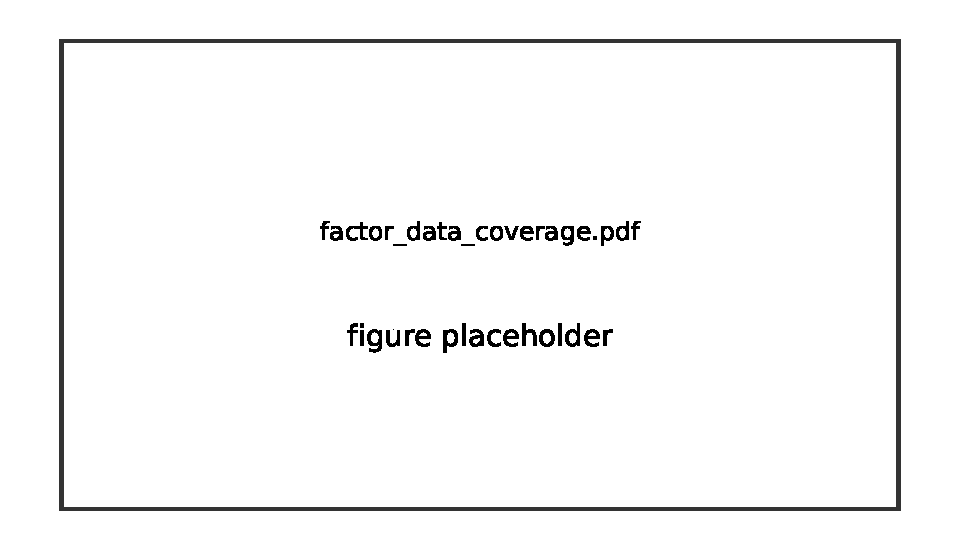
\includegraphics[width=\linewidth,height=0.62\textheight,keepaspectratio]{factor_data_coverage.pdf}
    \end{column}
    \begin{column}{0.32\textwidth}
      \small
      \keyterm{高覆盖}\par
      映射 100.00\%\par
      仓单 98.74\%\par
      2点曲线 98.37\%\par
      \medskip
      \riskterm{低覆盖}\par
      新鲜现货 73.41\%\par
      新鲜库存 33.95\%\par
      库存仅覆盖10个品种
    \end{column}
  \end{columns}
  \source{点时违规为0；库存类结果必须同步报告有效品种数。}
\end{frame}

% 07 — 25s
\begin{frame}{连续主力不能直接交易：映射到真实合约}
  \centering
  \begin{tikzpicture}[
    node distance=8mm,
    b/.style={draw=AcademicLine,fill=AcademicWhite,rounded corners=2pt,text width=31mm,minimum height=18mm,align=center,font=\small},
    a/.style={-{Stealth[length=2.2mm]},draw=AcademicNavy,thick}
  ]
    \node[b] (c) {\keyterm{连续主力序列}\par 描述长期走势\\但不可直接交易};
    \node[b,right=of c] (match) {\keyterm{逐字段匹配}\par pre-close / settle\\OHLC / 结算价};
    \node[b,right=of match] (real) {\keyterm{真实合约 $c$}\par 入场、持有、退出\\均锁定同一合约};
    \draw[a] (c)--node[above,font=\tiny]{T日收盘确认}(match);
    \draw[a] (match)--node[above,font=\tiny]{100\%覆盖}(real);
    \node[below=8mm of match,draw=AcademicRed,fill=AcademicRedSoft,rounded corners=2pt,text width=66mm,align=center,font=\scriptsize]
      {并列时依次使用：上一日合约连续性 $\rightarrow$ 持仓量 $\rightarrow$ 成交量 $\rightarrow$ 较晚到期日};
  \end{tikzpicture}
  \vfill
  \begin{takeaway}[避免的偏误]
    主力月份切换时，连续代码价格可能跳跃；真实合约映射避免把合约价差误当策略收益。
  \end{takeaway}
\end{frame}

% 08 — 25s
\begin{frame}{统一标签：收盘出信号，次日开盘进场，固定持有5日}
  \centering
  \begin{tikzpicture}[x=1.25cm,y=1cm]
    \draw[-{Stealth[length=2.4mm]},thick,AcademicNavy] (0,0)--(8.6,0);
    \foreach \x/\lab in {0/T,1/{T+1},2/{T+2},3/{T+3},4/{T+4},5/{T+5},6/{T+6}}{
      \draw[AcademicNavy] (\x,-.13)--(\x,.13);
      \node[below=2mm,font=\scriptsize] at (\x,0) {\lab};
    }
    \node[above=5mm,align=center,text=AcademicNavy,font=\small\bfseries] at (0,0) {收盘形成\\预测};
    \node[above=5mm,align=center,text=AcademicRed,font=\small\bfseries] at (1,0) {开盘\\建仓};
    \node[above=5mm,align=center,text=AcademicRed,font=\small\bfseries] at (6,0) {开盘\\平仓};
    \draw[AcademicRed,very thick] (1,.35)--node[above,font=\scriptsize]{同一真实合约 $c$，持有5个交易日}(6,.35);
  \end{tikzpicture}
  \vspace{5mm}
  \begin{equation*}
    y^{(5)}_{i,T}=\frac{Open_{c,T+6}}{Open_{c,T+1}}-1,
    \qquad \mathrm{label\_end\_date}_{5d}<\mathrm{valid\_start}
  \end{equation*}
  \begin{columns}[T,onlytextwidth]
    \begin{column}{0.48\textwidth}
      \begin{block}{防泄漏}
        时间有序训练并设置5日purge；验证标签结束日必须落在验证窗口内。
      \end{block}
    \end{column}
    \begin{column}{0.48\textwidth}
      \begin{alertblock}{实际修正}
        审计发现2个调仓日标签跨入2025，随后从头重算并降为0。
      \end{alertblock}
    \end{column}
  \end{columns}
\end{frame}

% 09 — 25s
\begin{frame}{样本外设计：七个扩展窗口，不随机划分}
  \centering
  \begin{tikzpicture}[x=.95cm,y=.52cm]
    \foreach \yr [count=\i from 0] in {2015,2016,2017,2018,2019,2020,2021,2022,2023,2024,2025}{
      \node[font=\tiny,rotate=45,anchor=east] at (\i,-.35) {\yr};
    }
    \foreach \test/\row in {4/6,5/5,6/4,7/3,8/2,9/1,10/0}{
      \fill[AcademicBlueSoft] (0,\row) rectangle (\test-.08,\row+.55);
      \fill[AcademicRed] (\test,\row) rectangle (\test+.82,\row+.55);
      \node[anchor=east,font=\tiny,text=AcademicNavy] at (-.15,\row+.27) {测试\pgfmathparse{2015+\test}\pgfmathprintnumber[precision=0]{\pgfmathresult}};
    }
    \node[font=\tiny,text=AcademicNavy] at (2,7) {历史训练区间逐年扩展};
    \node[font=\tiny,text=AcademicRed] at (8,7) {当年OOS};
  \end{tikzpicture}
  \vfill
  \begin{takeaway}[最终年度纪律]
    2025年只作为最终报告年度，不再用于反向修改因子方向、超参数范围或组合规则。
  \end{takeaway}
\end{frame}

% 10 — 25s
\begin{frame}{统一因子接口：57个概念因子变成92个字段}
  \begin{columns}[T,onlytextwidth]
    \begin{column}{0.48\textwidth}
      \centering
      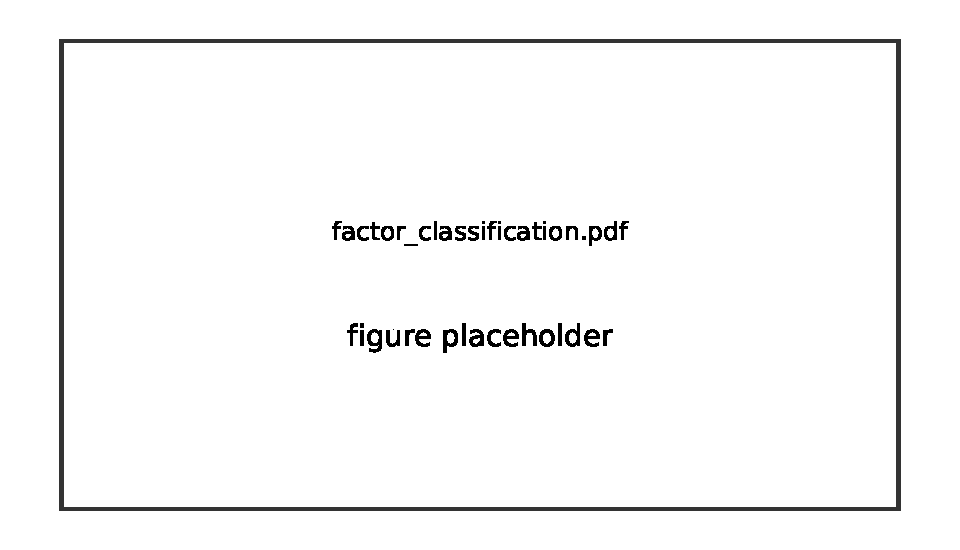
\includegraphics[width=0.82\linewidth,height=0.57\textheight,keepaspectratio]{factor_classification.pdf}
    \end{column}
    \begin{column}{0.48\textwidth}
      \begin{center}
        \metric{36}{预测因子}\hfill\metric{45}{质量标志}
      \end{center}
      \smallskip
      \small
      另含5个条件变量、6个风险变量；92字段形成65个相关性簇。缺失值在数值输入中置为中性0，同时保留可用性标志。
      \medskip
      \begin{alertblock}{解释边界}
        质量标志可帮助预测，但通常代表覆盖、上市阶段或更新规律，\riskterm{不能解释为新Alpha}。
      \end{alertblock}
    \end{column}
  \end{columns}
\end{frame}

% 11 — 25s
\begin{frame}{因子层结果：期限结构和供需信息相对更强}
  \begin{columns}[T,onlytextwidth]
    \begin{column}{0.68\textwidth}
      \centering
      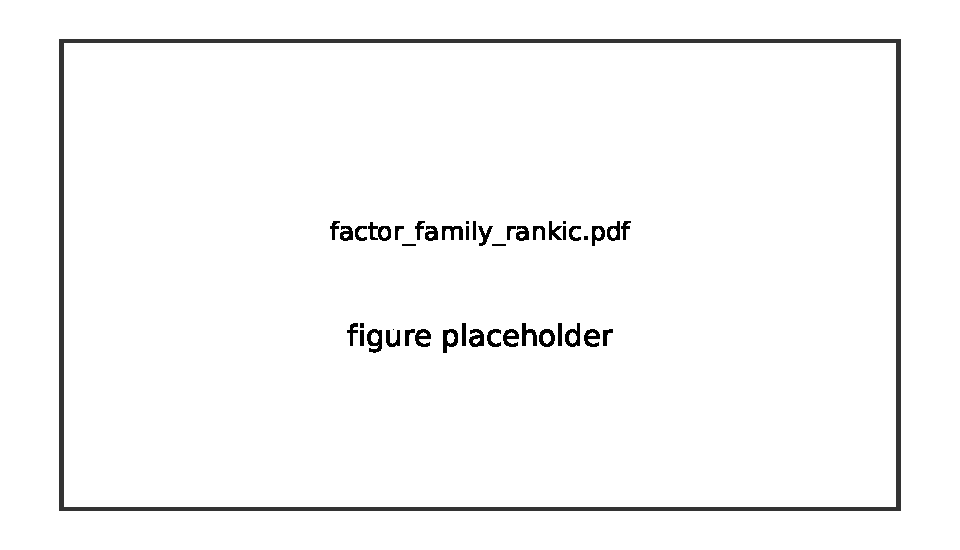
\includegraphics[width=\linewidth,height=0.61\textheight,keepaspectratio]{factor_family_rankic.pdf}
    \end{column}
    \begin{column}{0.28\textwidth}
      \small
      \keyterm{家族平均Rank IC}\par
      库存与供需 0.0183\par
      非线性交互 0.0143\par
      信息类 0.0112\par
      期限结构 0.0108\par
      \medskip
      \riskterm{总体偏弱或为负}\par
      趋势动量、波动风险、产业链代理
    \end{column}
  \end{columns}
  \source{期限结构、基差和库存约束具有经济解释，但仍属于弱预测信号。}
\end{frame}

% 12 — 25s
\begin{frame}{没有“核心Alpha”：8个B类候选，0个A类因子}
  \begin{columns}[T,onlytextwidth]
    \begin{column}{0.49\textwidth}
      \centering
      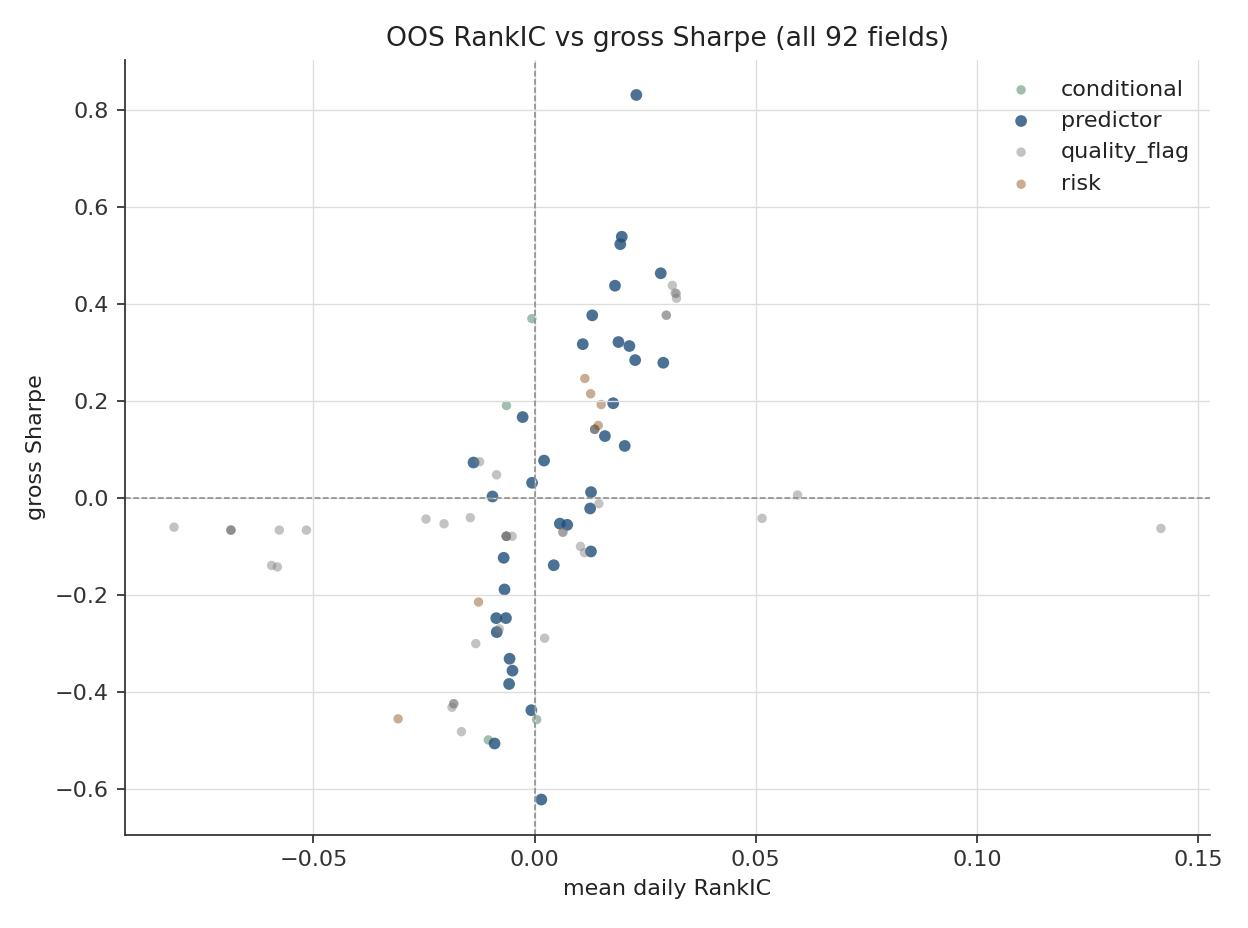
\includegraphics[width=\linewidth,height=0.49\textheight,keepaspectratio]{factor_ic_vs_sharpe.pdf}
      \scriptsize 预测能力与5bps可交易性
    \end{column}
    \begin{column}{0.49\textwidth}
      \centering
      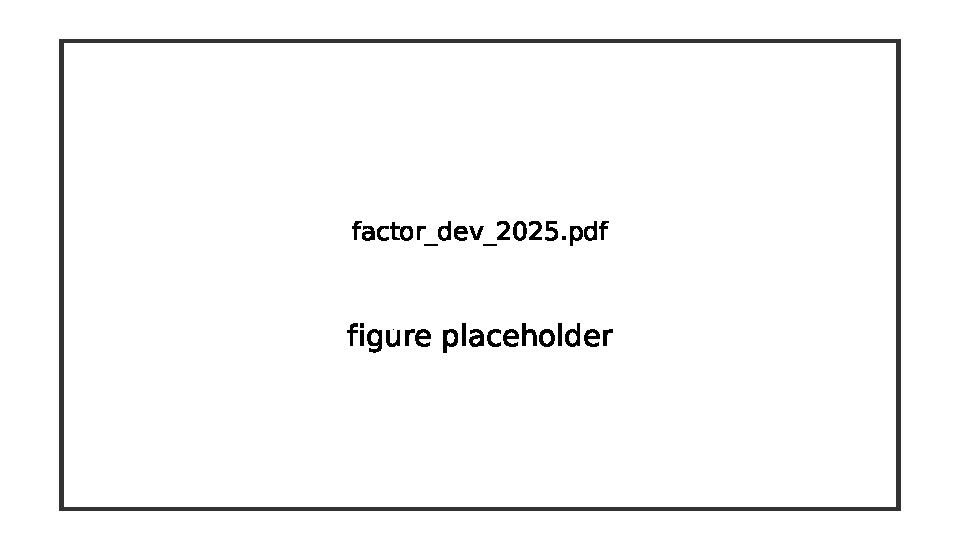
\includegraphics[width=\linewidth,height=0.49\textheight,keepaspectratio]{factor_dev_2025.pdf}
      \scriptsize 最终年度方向持续性
    \end{column}
  \end{columns}
  \vfill
  \begin{takeaway}[A类三道门槛]
    Rank IC $\ge 0.02$、5bps年化收益为正、全库FDR $q\le0.10$；最终\riskterm{没有因子同时通过}。
  \end{takeaway}
\end{frame}

% 13 — 30s
\begin{frame}{成本是第一道分水岭：单因子优势几乎被吃掉}
  \begin{columns}[T,onlytextwidth]
    \begin{column}{0.66\textwidth}
      \centering
      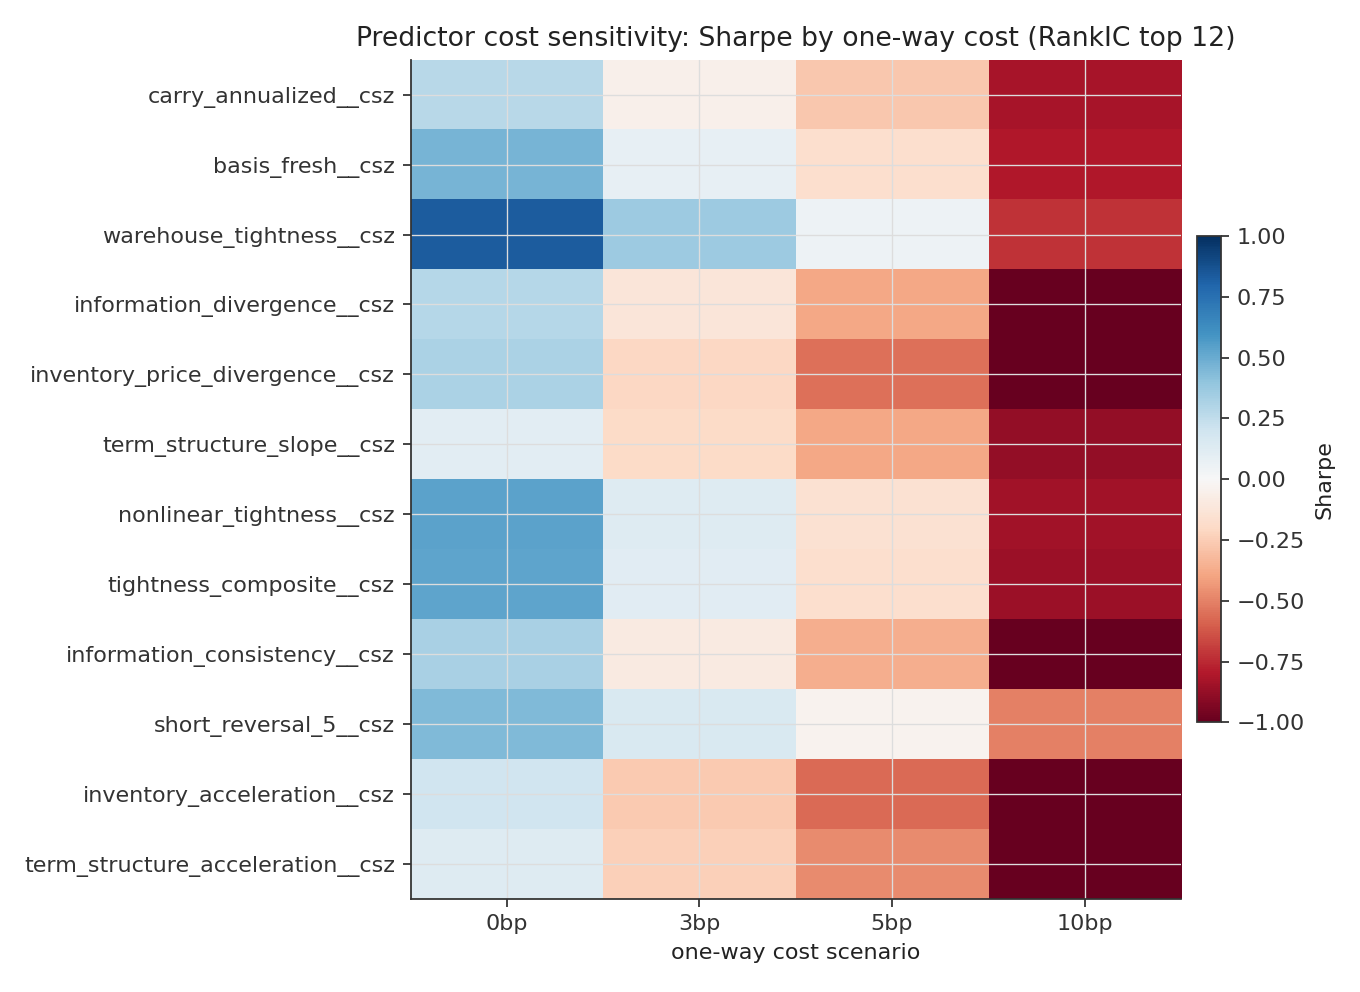
\includegraphics[width=\linewidth,height=0.60\textheight,keepaspectratio]{single_factor_cost.png}
    \end{column}
    \begin{column}{0.30\textwidth}
      \small
      \keyterm{36个predictor}\par
      Rank IC中位数 0.0065\par
      5bps年化中位数 $-4.89\%$\par
      5bps Sharpe中位数 $-0.577$\par
      \medskip
      \riskterm{仅1个因子}\par
      在5bps下净Sharpe为正
    \end{column}
  \end{columns}
  \source{仓单紧张度：3bps年化2.36\%、Sharpe 0.364；5bps仅0.34\%、Sharpe 0.053。}
\end{frame}

% 14 — 30s
\begin{frame}{统一执行引擎：模型只负责输出预测分数}
  \centering
  \begin{tikzpicture}[
    model/.style={draw=AcademicLine,fill=AcademicWhite,rounded corners=2pt,text width=22mm,minimum height=9mm,align=center,font=\scriptsize},
    engine/.style={draw=AcademicNavy,very thick,fill=AcademicBlueSoft,rounded corners=2pt,text width=35mm,minimum height=18mm,align=center,font=\small},
    a/.style={-{Stealth[length=1.8mm]},draw=AcademicNavy}
  ]
    \node[model] (s1) at (0,2.3) {单因子 / 等权};
    \node[model] (s2) at (0,1.1) {Ridge};
    \node[model] (s3) at (0,-.1) {LightGBM / XGB / RF};
    \node[model] (s4) at (0,-1.3) {HCGNN};
    \node[model] (s5) at (0,-2.5) {Conv--Transformer};
    \node[engine] (e) at (4.5,-.1) {\keyterm{统一预测接口}\par \texttt{date, product, score}};
    \node[engine] (p) at (9,-.1) {\keyterm{统一执行引擎}\par 排序、持仓、换手、成本、净值};
    \foreach \s in {s1,s2,s3,s4,s5}{\draw[a] (\s.east)--(e.west);}
    \draw[a,very thick] (e)--(p);
  \end{tikzpicture}
  \vfill
  \small \tagbox{每5日调仓}\quad \tagbox{至少8个品种}\quad \tagbox{多空各20\%}\quad \tagbox{两侧权重各0.5}\quad \redtag{主成本5bps}
\end{frame}

% 15 — 30s
\begin{frame}{等权与Ridge：Rank IC提高，但没有覆盖成本}
  \begin{columns}[T,onlytextwidth]
    \begin{column}{0.58\textwidth}
      \centering
      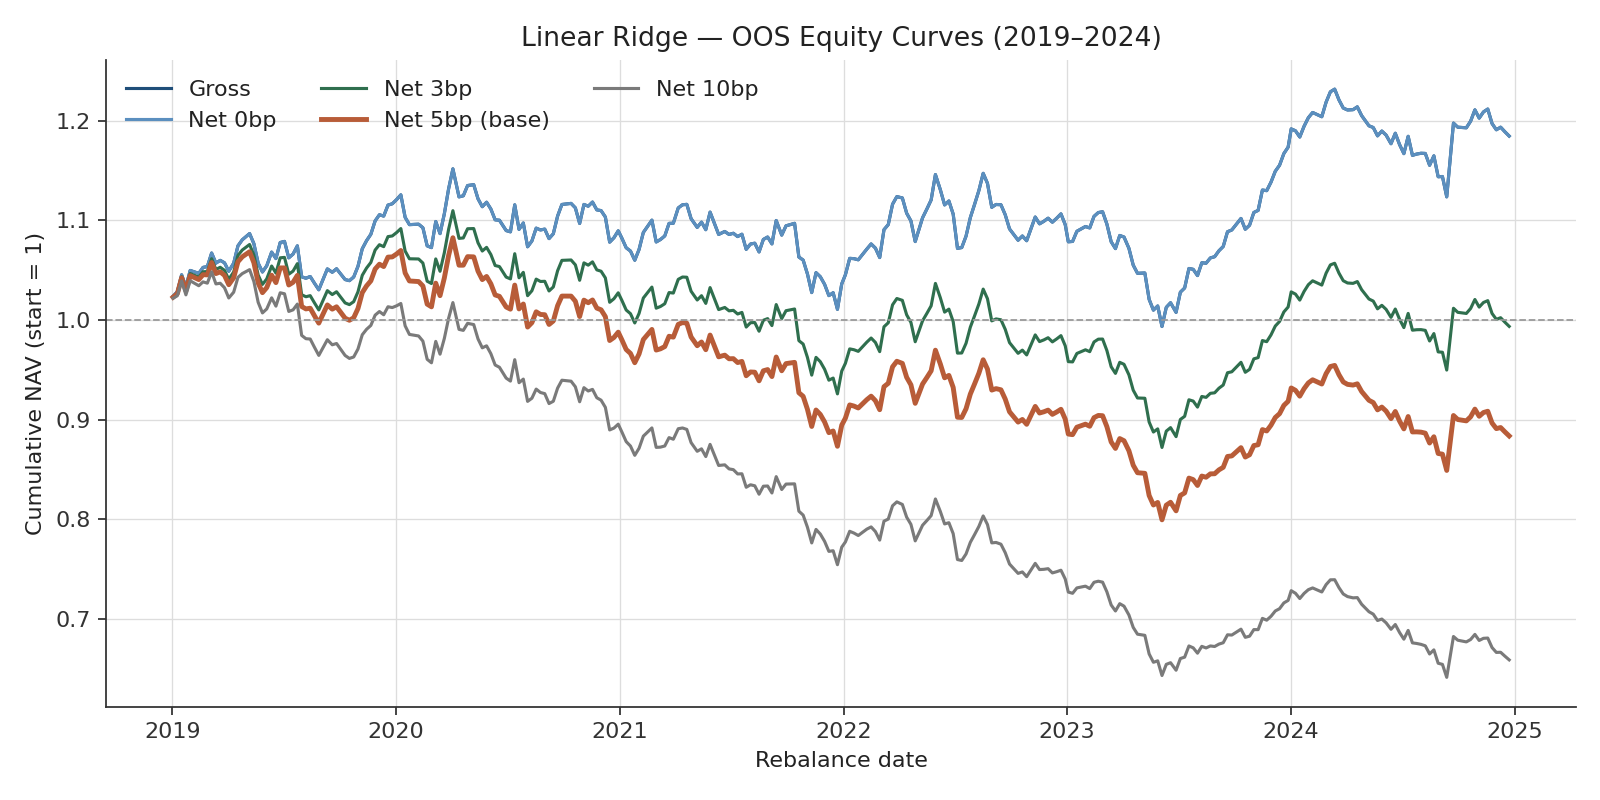
\includegraphics[width=\linewidth,height=0.48\textheight,keepaspectratio]{ridge_equity.png}
      \scriptsize Ridge毛收益与成本后净值
    \end{column}
    \begin{column}{0.38\textwidth}
      \small
      \begin{tabular}{lrr}
        \toprule
         & 等权 & Ridge \\
        \midrule
        Rank IC & 0.0163 & \textbf{0.0247} \\
        毛Sharpe & 0.358 & \textbf{0.397} \\
        5bps Sharpe & -0.216 & -0.219 \\
        5bps年化 & -1.88\% & -1.79\% \\
        \bottomrule
      \end{tabular}
      \medskip
      \begin{alertblock}{解释}
        数据驱动权重有\keyterm{预测增量}，但增量不足以覆盖同一调仓协议下的摩擦。
      \end{alertblock}
    \end{column}
  \end{columns}
  \source{Ridge每折只在训练窗口末年从 $\alpha\in\{0.01,0.1,1,10,100\}$ 中选参。}
\end{frame}

% 16 — 30s
\begin{frame}{正则化树模型：能表达非线性，不等于获得经济增量}
  \begin{columns}[T,onlytextwidth]
    \begin{column}{0.57\textwidth}
      \small
      \begin{tabular}{lrrrr}
        \toprule
        模型 & Rank IC & 5bps年化 & Sharpe & 换手 \\
        \midrule
        LightGBM & 0.0184 & -2.12\% & -0.213 & 21.56\% \\
        随机森林 & -0.0006 & -5.96\% & -0.628 & 22.55\% \\
        XGBoost & -0.0025 & -1.53\% & -0.134 & 20.44\% \\
        \bottomrule
      \end{tabular}
      \medskip
      \begin{alertblock}{稳定性门槛未通过}
        LightGBM的5bps HAC检验 $p=0.596$；三种树模型均未同时达到多数年度Rank IC为正、净Sharpe为正和统计显著。
      \end{alertblock}
    \end{column}
    \begin{column}{0.39\textwidth}
      \centering
      \begin{tikzpicture}[x=.65cm,y=.55cm]
        \draw[->,AcademicMuted] (0,0)--(6.5,0) node[right,font=\tiny]{5bps年化};
        \draw[->,AcademicMuted] (3,-.3)--(3,5.1);
        \foreach \y/\name/\v in {4.2/LightGBM/-2.12,2.7/XGBoost/-1.53,1.2/随机森林/-5.96}{
          \node[anchor=east,font=\scriptsize] at (2.8,\y) {\name};
          \fill[AcademicRed] ({3+0.42*\v},\y-.18) rectangle (3,\y+.18);
          \node[anchor=east,font=\tiny,text=AcademicRed] at ({3+0.42*\v-.1},\y) {\v\%};
        }
      \end{tikzpicture}
      \scriptsize 即使0bps，LightGBM/XGBoost年化也仅0.57\% / 1.03\%。
    \end{column}
  \end{columns}
\end{frame}

% 17 — 30s
\begin{frame}{HCGNN：当前图关系设定呈现较低换手优势}
  \begin{columns}[T,onlytextwidth]
    \begin{column}{0.49\textwidth}
      \small
      \begin{tabular}{lrr}
        \toprule
         & HCGNN持续 & 协议GNN \\
        \midrule
        Rank IC & 0.0193 & \textbf{0.0226} \\
        5bps年化 & \textbf{3.11\%} & 2.73\% \\
        Sharpe & \textbf{0.454} & 0.413 \\
        最大回撤 & \textbf{-13.44\%} & -15.75\% \\
        日均换手 & \textbf{7.23\%} & 9.21\% \\
        \bottomrule
      \end{tabular}
      \medskip
      \begin{takeaway}[当前设定下的结果]
        协议GNN排序更高；持续学习版因换手更低，在当前图关系定义下获得更好的净收益与回撤。
      \end{takeaway}
    \end{column}
    \begin{column}{0.47\textwidth}
      \centering
      \begin{tikzpicture}[x=.68cm,y=.7cm]
        \draw[->,AcademicMuted] (0,0)--(7,0) node[right,font=\tiny]{成本};
        \draw[->,AcademicMuted] (0,0)--(0,5.1) node[above,font=\tiny]{年化\%};
        \draw[AcademicNavy,very thick] plot coordinates {(0,4.05) (2,3.49) (3.33,3.11) (6.67,2.18)};
        \foreach \x/\y/\lab in {0/4.05/0bps,2/3.49/3bps,3.33/3.11/5bps,6.67/2.18/10bps}{
          \fill[AcademicRed] (\x,\y) circle (2pt);
          \node[above,font=\tiny] at (\x,\y) {\y\%};
          \node[below,font=\tiny] at (\x,0) {\lab};
        }
      \end{tikzpicture}
      \scriptsize 当前结构化图设定呈现组合增量；精确产业邻接与生产配比仍待冻结。
    \end{column}
  \end{columns}
\end{frame}

% Transformer专题 1
\begin{frame}{Transformer迭代（一）：先承认早期模型“不像交易”}
  \begin{columns}[T,onlytextwidth]
    \begin{column}{0.57\textwidth}
      \centering
      
\includegraphics[width=\linewidth,height=0.52\textheight,keepaspectratio]{v1_loss_curve.png}
      \scriptsize 早期1D--CNN：若干验证损失近似横线，训练收敛不等于有效学习
    \end{column}
    \begin{column}{0.39\textwidth}
      \small
      \begin{alertblock}{观察到的症状}
        \begin{itemize}
          \item 目标是\riskterm{次日收益}，噪声强、可预测成分弱；
          \item 验证loss很快变平，网络接近输出常数；
          \item 训练曲线稳定下降，但样本外净值长期下行；
          \item 毛收益本就偏弱，费用进一步放大亏损。
        \end{itemize}
      \end{alertblock}
    \end{column}
  \end{columns}
  \vfill
  \begin{takeaway}[问题判断]
    失败不只是“参数没调好”：标签、验证和组合规则离真实交易太远，同时有限横截面让深度网络严重过拟合。
  \end{takeaway}
\end{frame}

% Transformer专题 2
\begin{frame}{Transformer迭代（二）：从拟合模型转向可交易研究系统}
  \centering
  \begin{tikzpicture}[
    node distance=4.5mm,
    st/.style={draw=AcademicLine,fill=AcademicWhite,rounded corners=2pt,text width=25mm,minimum height=16mm,align=center,font=\scriptsize},
    ar/.style={-{Stealth[length=1.9mm]},draw=AcademicNavy,thick}
  ]
    \node[st] (s1) {\keyterm{V1 基线}\par 5因子·1D--CNN\\次日标签};
    \node[st,right=of s1] (s2) {\keyterm{V3/V4 交易化}\par 5日标签·扩展窗口\\EMA·持仓缓冲·GMM};
    \node[st,right=of s2] (s3) {\keyterm{V5 表示升级}\par Conv局部模式\\单层注意力·双头任务};
    \node[st,right=of s3] (s4) {\keyterm{V6 正则强化}\par 59维输入\\Dropout 0.40·低换手};
    \draw[ar] (s1)--(s2); \draw[ar] (s2)--(s3); \draw[ar] (s3)--(s4);
  \end{tikzpicture}
  \vspace{4mm}
  \begin{columns}[T,onlytextwidth]
    \begin{column}{0.48\textwidth}
      \begin{block}{训练端：抑制过拟合}
        \begin{itemize}
          \item 轻量单层Transformer：4头、48维表示、96维FFN；
          \item 分类+Huber回归双头，降低极端收益主导；
          \item Dropout由0.10提高至0.40，权重衰减提高至$10^{-3}$；
          \item 最多40轮、patience=7早停，时间验证与purge。
        \end{itemize}
      \end{block}
    \end{column}
    \begin{column}{0.48\textwidth}
      \begin{block}{交易端：靠近实盘}
        \begin{itemize}
          \item 3日EMA平滑、入场/退出宽缓冲带；
          \item 最低20\%流动性准入，降低不可成交风险；
          \item GMM压力状态降杠杆，控制回撤；
          \item 成本直接进入评价，关注净收益而非训练loss。
        \end{itemize}
      \end{block}
    \end{column}
  \end{columns}
  \vfill
  \source{核心思路：数据契约、时间验证和执行约束，比继续堆叠Transformer层数更重要。}
\end{frame}

% Transformer专题 3
\begin{frame}{Transformer迭代（三）：更复杂不是终点，稳健路径才是}
  \begin{columns}[T,onlytextwidth]
    \begin{column}{0.48\textwidth}
      \centering
      
\includegraphics[width=\linewidth,height=0.46\textheight,keepaspectratio]{v5_loss_curve.png}
      \scriptsize V5：训练loss继续下降，部分验证折后期回升\par
      \redtag{用早停而非继续训练}
    \end{column}
    \begin{column}{0.48\textwidth}
      \centering
      
\includegraphics[width=\linewidth,height=0.46\textheight,keepaspectratio]{v6_fee_sensitivity.png}
      \scriptsize V6：费用曲线间距收窄，主要来自换手下降\par
      \tagbox{日均换手 0.141 $\rightarrow$ 0.076}
    \end{column}
  \end{columns}
  \vspace{2mm}
  \small
  \begin{tabular}{lrrr}
    \toprule
    历史版本（不同协议） & 毛年化 & 3bps年化 & 5bps年化 \\
    \midrule
    V3：1D--CNN & -3.41\% & -5.55\% & -6.9\% \\
    V5：Conv--Transformer & 2.51\% & 0.35\% & -1.06\% \\
    V6：59维 + 强正则 & 1.96\% & 0.80\% & 0.03\% \\
    \bottomrule
  \end{tabular}
  \vfill
  \begin{takeaway}[审慎结论]
    历史结果说明“更长标签+多任务表示+正则化+低换手执行”值得继续研究，但版本协议不同，\riskterm{不能把全部改善单独归因于Transformer}。
  \end{takeaway}
\end{frame}

% 18 — 30s
\begin{frame}{Conv--Transformer：路径为正，但证据尚不显著}
  \begin{columns}[T,onlytextwidth]
    \begin{column}{0.47\textwidth}
      \centering
      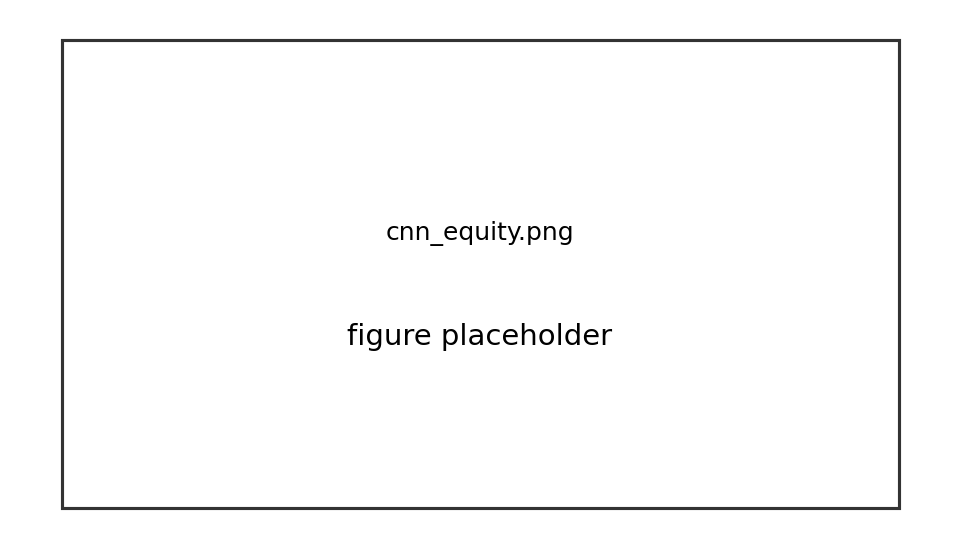
\includegraphics[width=\linewidth,height=0.50\textheight,keepaspectratio]{cnn_equity.png}
      \scriptsize 5bps净值与回撤
    \end{column}
    \begin{column}{0.47\textwidth}
      \centering
      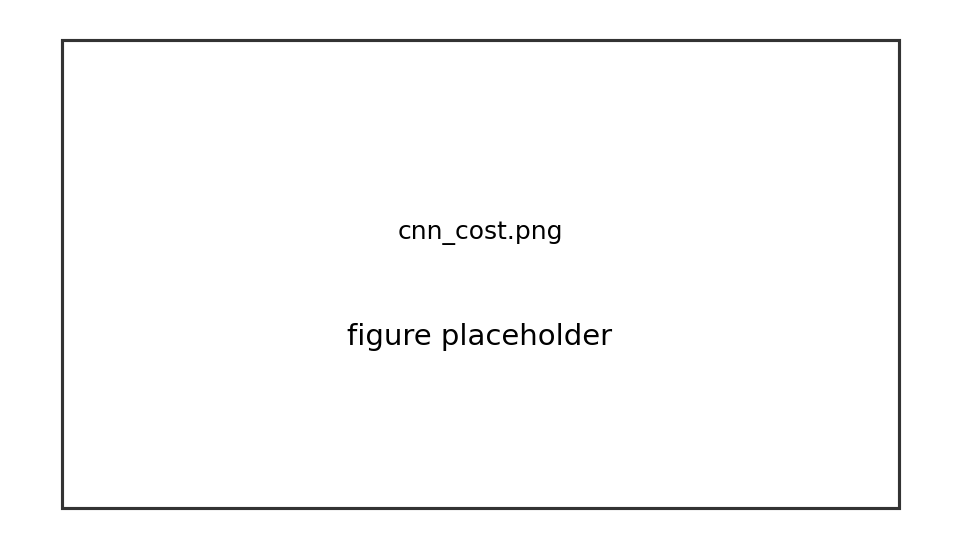
\includegraphics[width=\linewidth,height=0.50\textheight,keepaspectratio]{cnn_cost.png}
      \scriptsize 成本敏感性
    \end{column}
  \end{columns}
  \vfill
  \small \tagbox{Rank IC 0.0069}\quad \tagbox{5bps年化 1.14\%}\quad \tagbox{Sharpe 0.185}\quad \redtag{HAC $p=0.636$}\quad \redtag{2024 Rank IC -0.0752}
\end{frame}

% 19 — 25s
\begin{frame}{统一成绩单：真正拉开差距的是成本承受力}
  \begin{columns}[T,onlytextwidth]
    \begin{column}{0.63\textwidth}
      \small
      \begin{tabular}{lrrr}
        \toprule
        策略 & Rank IC & 5bps年化 & 5bps Sharpe \\
        \midrule
        HCGNN持续学习 & 0.0193 & \textbf{3.11\%} & \textbf{0.454} \\
        Conv--Transformer & 0.0069 & 1.14\% & 0.185 \\
        仓单紧张度 & $\sim$0.023 & 0.34\% & 0.053 \\
        Ridge & \textbf{0.0247} & -1.79\% & -0.219 \\
        等权多因子 & 0.0163 & -1.88\% & -0.216 \\
        LightGBM & 0.0184 & -2.12\% & -0.213 \\
        \bottomrule
      \end{tabular}
    \end{column}
    \begin{column}{0.33\textwidth}
      \centering
      \begin{tikzpicture}[x=1cm,y=.95cm]
        \draw[->,AcademicMuted] (0,0)--(3.5,0) node[right,font=\tiny]{Rank IC};
        \draw[->,AcademicMuted] (0,0)--(0,3.6) node[above,font=\tiny]{净Sharpe};
        \fill[AcademicNavy] (2.35,2.85) circle (5pt) node[right,font=\tiny]{HCGNN};
        \fill[AcademicNavy!65] (.85,1.75) circle (4pt) node[right,font=\tiny]{Conv};
        \fill[AcademicRed] (3.0,.45) circle (4pt) node[right,font=\tiny]{Ridge};
        \fill[AcademicRed!70] (2.0,.46) circle (4pt) node[right,font=\tiny]{等权};
        \draw[AcademicMuted,dashed] (0,1.15)--(3.4,1.15);
      \end{tikzpicture}
      \scriptsize 最高Rank IC并不对应最高净Sharpe。
    \end{column}
  \end{columns}
  \vfill
  \begin{takeaway}[模型比较结论]
    当前图关系定义下，HCGNN的相对优势来自结构化预测与低换手的共同作用；该结果不代表已验证完整产业链真值。
  \end{takeaway}
\end{frame}

% 20 — 25s
\begin{frame}{跨年漂移与信息衰减：平均结果掩盖不稳定}
  \begin{columns}[T,onlytextwidth]
    \begin{column}{0.62\textwidth}
      \centering
      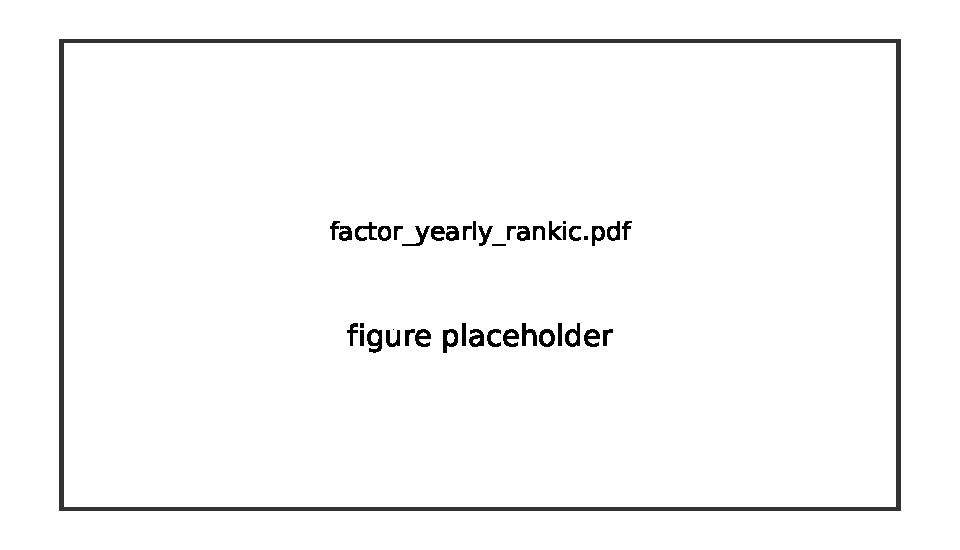
\includegraphics[width=\linewidth,height=0.55\textheight,keepaspectratio]{factor_yearly_rankic.pdf}
      \scriptsize 2019--2025年度Rank IC
    \end{column}
    \begin{column}{0.34\textwidth}
      \centering
      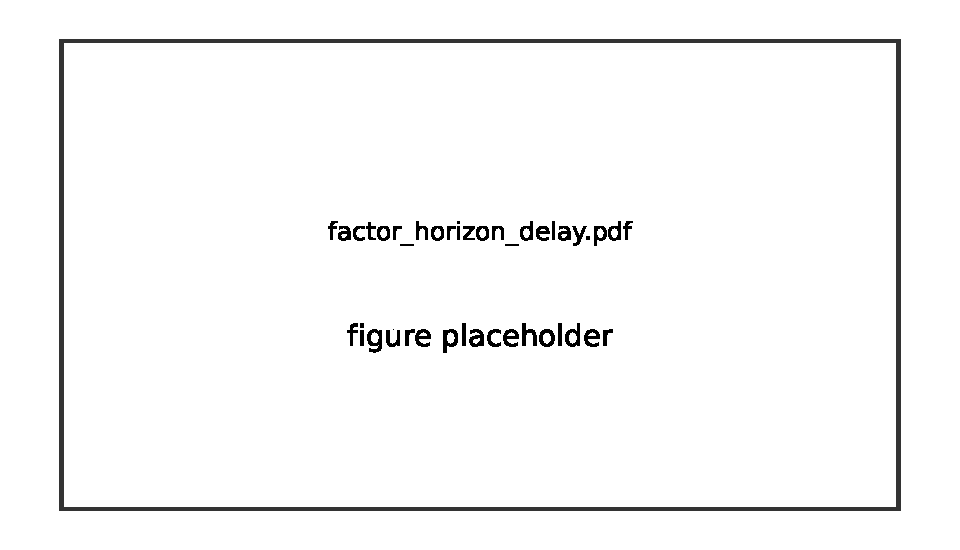
\includegraphics[width=\linewidth,height=0.30\textheight,keepaspectratio]{factor_horizon_delay.pdf}
      \scriptsize 期限与延迟
      \medskip
      \begin{alertblock}{失效证据}
        因子同方向比例仅37.5\%；Conv信号延迟一天由0.0069降至0.0054；部分库存与信息因子在2025反向。
      \end{alertblock}
    \end{column}
  \end{columns}
\end{frame}

% 21 — 25s
\begin{frame}{四个假设的回答}
  \begin{columns}[T,onlytextwidth]
    \begin{column}{0.48\textwidth}
      \begin{block}{H1 弱信号｜部分支持}
        库存供需家族Rank IC约0.0183，但严格A类因子数量为0。
      \end{block}
      \begin{block}{H2 组合改善｜预测层支持}
        Ridge Rank IC 0.0247，高于等权0.0163；结构模型进一步改善组合路径。
      \end{block}
    \end{column}
    \begin{column}{0.48\textwidth}
      \begin{alertblock}{H3 成本侵蚀｜明确支持}
        Ridge在5bps下年化$-1.79\%$；Conv在10bps下年化$-0.32\%$。
      \end{alertblock}
      \begin{alertblock}{H4 治理约束｜过程支持}
        两个跨界调仓日、两套主力规则与单位不可比数据均足以改变最终叙事。
      \end{alertblock}
    \end{column}
  \end{columns}
  \vfill
  \keyterm{综合判断：}机器学习价值成立在部分预测与组合层，但成本和治理决定这种价值能否被相信、能否被交易。
\end{frame}

% 22 — 20s
\begin{frame}{AI的真实价值是工程化，真实风险是静默改协议}
  \begin{columns}[T,onlytextwidth]
    \begin{column}{0.48\textwidth}
      \begin{block}{AI加速了什么？}
        \begin{itemize}
          \item 数据字段识别与清洗脚本
          \item 57个因子、92字段接口实现
          \item 多模型、多窗口、多成本批量实验
          \item 图表、文档整合与错误检索
        \end{itemize}
      \end{block}
    \end{column}
    \begin{column}{0.48\textwidth}
      \begin{alertblock}{AI可能悄悄改变什么？}
        \begin{itemize}
          \item 至少两套“主力合约”定义
          \item 自动填充导致的点时泄漏
          \item FU、I、SC单位/汇率不可比
          \item 结果文件与报告口径漂移
        \end{itemize}
      \end{alertblock}
    \end{column}
  \end{columns}
  \vfill
  \begin{takeaway}[项目经验]
    最危险的AI错误不是代码报错，而是代码正常运行、研究协议却已经悄悄改变。
  \end{takeaway}
\end{frame}

% 23 — 20s
\begin{frame}{治理与局限：哪些已完成，哪些尚不能声称}
  \centering
  \begin{tikzpicture}[
    node distance=4mm,
    done/.style={draw=AcademicNavy,fill=AcademicBlueSoft,rounded corners=2pt,text width=25mm,minimum height=10mm,align=center,font=\scriptsize},
    todo/.style={draw=AcademicRed,fill=AcademicRedSoft,rounded corners=2pt,text width=28mm,minimum height=10mm,align=center,font=\scriptsize}
  ]
    \node[done] (d1) {协议冻结与版本号};
    \node[done,right=of d1] (d2) {核心TuShare血缘\\与时间边界};
    \node[done,right=of d2] (d3) {Schema / 经济恒等式};
    \node[done,right=of d3] (d4) {交接包哈希核验};
    \node[todo,below=8mm of d1] (t1) {商业数据字段级血缘};
    \node[todo,right=of t1] (t2) {最终年度独立复核};
    \node[todo,right=of t2] (t3) {涨跌停与换月冲击};
    \node[todo,right=of t3] (t4) {完整真实费率覆盖};
  \end{tikzpicture}
  \vfill
  \small \redtag{真实手续费覆盖约73.16\%}\quad \redtag{库存10/30品种}\quad \redtag{现货止于2023-12-29}\quad \redtag{换月额外冲击当前为0}
  \medskip
  \begin{takeaway}[证据边界]
    当前结果属于\keyterm{严格研究回测}，不是完整实盘模拟；未完成项必须对所有模型统一补齐后再比较。
  \end{takeaway}
\end{frame}

% 24 — 20s
\begin{frame}[plain]
  \begin{tikzpicture}[remember picture,overlay]
    \fill[AcademicNavy] (current page.south west) rectangle (current page.north east);
    \fill[AcademicRed] ([xshift=-13mm,yshift=13mm]current page.south east) circle (2.5mm);
  \end{tikzpicture}
  \vspace*{5mm}
  \begin{minipage}{0.95\textwidth}
  {\color{AcademicIvory}\fontsize{23}{28}\selectfont\bfseries 最可信的贡献：一套可审计的研究基座\par}
  \vspace{7mm}
  \begin{columns}[T,onlytextwidth]
    \begin{column}{0.30\textwidth}
      {\color{AcademicIvory}\bfseries 01 弱信号整合\par}
      \smallskip{\color{AcademicIvory!80}\small ML能改善部分横截面排序，但0个因子通过严格三重门槛。}
    \end{column}
    \begin{column}{0.30\textwidth}
      {\color{AcademicIvory}\bfseries 02 成本决定落地\par}
      \smallskip{\color{AcademicIvory!80}\small 最高Rank IC不等于最高净Sharpe，低换手是结构模型的关键。}
    \end{column}
    \begin{column}{0.30\textwidth}
      {\color{AcademicIvory}\bfseries 03 协议决定可信度\par}
      \smallskip{\color{AcademicIvory!80}\small 数据血缘、点时边界和AI复核比模型新颖性更重要。}
    \end{column}
  \end{columns}
  \vspace{12mm}
  {\color{AcademicIvory!92}\large 复杂度不是免费的午餐；统一协议与交易可实现性，才是可信增量的前提。\par}
  \vspace{5mm}
  {\color{AcademicIvory!70}\small 谢谢各位老师与同学。}
  \end{minipage}
\end{frame}

% ==================== BACKUP: 11 slides ====================
\appendix

% 25
\begin{frame}{备份｜核心因子如何定义？}
  \small
  \begin{tabularx}{\textwidth}{@{}p{2.2cm}Xp{3.0cm}@{}}
    \toprule
    \keyterm{因子} & \keyterm{定义} & \keyterm{经济含义} \\
    \midrule
    TSMOM 60 & $\log(P_t/P_{t-60})/(\sigma_{60}\sqrt{60})$ & 风险调整趋势 \\
    Carry & $\log(F_1/F_2)\,365/\Delta\tau$ & Backwardation溢价 \\
    新鲜基差 & $(S_t^{fresh}-F_t^{main})/F_t^{main}$ & 现货紧张度 \\
    仓单紧张度 & 注册仓单季节Z分数取负 & 可交割供给约束 \\
    库存变化 & 5期库存变化取负 & 边际去库信息 \\
    Amihud & 20日均值$\{|r|/\mathrm{amount}\}$ & 流动性风险 \\
    \bottomrule
  \end{tabularx}
  \vfill
  \begin{block}{点时门槛}
    现货、仓单、库存统一至少延迟1个交易日，最大陈旧期分别为7、5、14个自然日；期限点剩余10--365日且成交或持仓占比至少1\%。
  \end{block}
\end{frame}

% 26
\begin{frame}{备份｜真实合约映射与点时安全}
  \begin{columns}[T,onlytextwidth]
    \begin{column}{0.55\textwidth}
      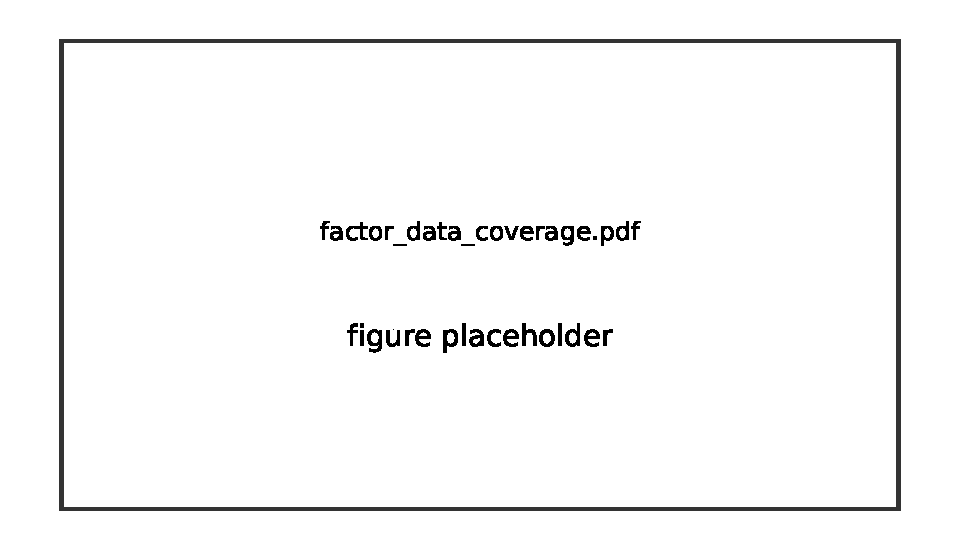
\includegraphics[width=\linewidth,height=0.58\textheight,keepaspectratio]{factor_data_coverage.pdf}
    \end{column}
    \begin{column}{0.41\textwidth}
      \small
      \keyterm{审计结果}\par
      映射覆盖 100\%\par
      高质量匹配 99\%\par
      点时违规 0\par
      \medskip
      \riskterm{保留限制}\par
      TuShare未公开连续主力选择算法及日内确定时间，因此不能无条件声称该身份在当日开盘前可知。信号放在T日收盘、T+1开盘交易以降低风险。
    \end{column}
  \end{columns}
\end{frame}

% 27
\begin{frame}{备份｜七个扩展窗口的完整定义}
  \centering
  \small
  \begin{tabular}{cccc}
    \toprule
    测试年 & 训练区间 & 测试区间 & Purge \\
    \midrule
    2019 & 2015-01-05--2018-12-31 & 2019全年 & 5日 \\
    2020 & 2015-01-05--2019-12-31 & 2020全年 & 5日 \\
    2021 & 2015-01-05--2020-12-31 & 2021全年 & 5日 \\
    2022 & 2015-01-05--2021-12-31 & 2022全年 & 5日 \\
    2023 & 2015-01-05--2022-12-31 & 2023全年 & 5日 \\
    2024 & 2015-01-05--2023-12-31 & 2024全年 & 5日 \\
    2025 & 2015-01-05--2024-12-31 & 2025全年 & 5日 \\
    \bottomrule
  \end{tabular}
  \vfill
  \begin{takeaway}[为什么不用随机划分？]
    金融特征关系时变；随机打乱会把未来状态混入训练。扩展窗口模拟研究者逐年获得新数据的真实过程。
  \end{takeaway}
\end{frame}

% 28
\begin{frame}{备份｜8个B类候选因子的完整结果}
  \scriptsize
  \centering
  \begin{tabular}{lrrrrrr}
    \toprule
    因子 & OOS Rank IC & FDR q & 5bps年化 & Sharpe & 2025 Rank IC & 2025年化 \\
    \midrule
    Carry & 0.0293 & 0.1931 & 3.2\% & 0.369 & 0.0323 & 2.9\% \\
    新鲜基差 & 0.0309 & 0.1926 & 6.7\% & 0.741 & -- & -- \\
    库存变化 & 0.0211 & 0.4592 & 5.9\% & 0.656 & -0.0557 & -9.0\% \\
    仓单紧张度 & 0.0236 & 0.1926 & 3.8\% & 0.524 & 0.0653 & 3.7\% \\
    信息背离 & 0.0257 & 0.2816 & 2.7\% & 0.371 & -0.1062 & -20.9\% \\
    期限结构斜率 & 0.0241 & 0.4274 & 3.6\% & 0.349 & 0.0165 & -2.3\% \\
    库存加速度 & 0.0316 & 0.1926 & 4.3\% & 0.473 & 0.0136 & 2.7\% \\
    库存--价格背离 & 0.0315 & 0.2316 & 4.7\% & 0.536 & -0.0836 & -18.5\% \\
    \bottomrule
  \end{tabular}
  \begin{minipage}{0.96\textwidth}\tiny\color{AcademicMuted}
    注：本表来自因子筛选管线；仓单紧张度在统一单因子基准中另有5bps年化0.34\%、Sharpe 0.053。两条管线的方向冻结与执行细节尚待回到底表统一，不能直接横比。
  \end{minipage}
  \vfill
  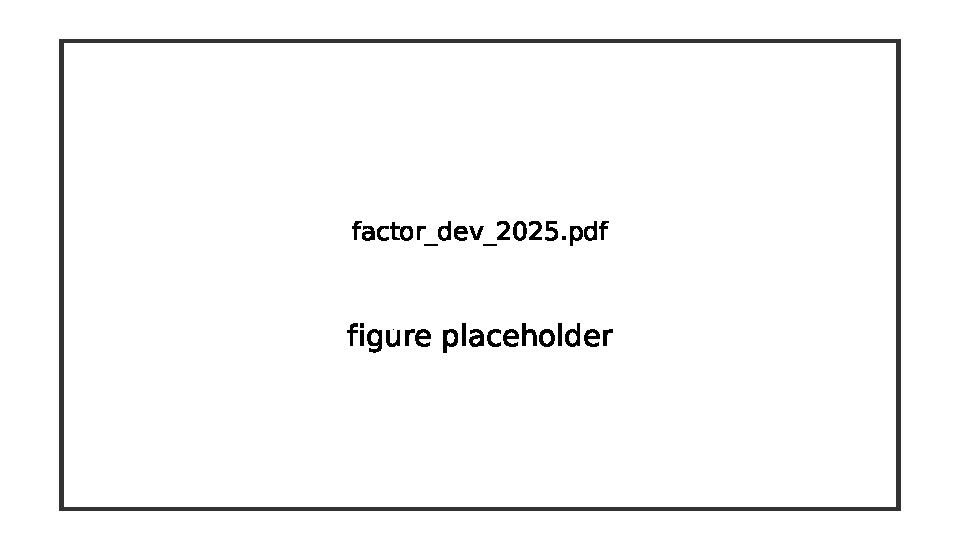
\includegraphics[width=0.52\linewidth,height=0.29\textheight,keepaspectratio]{factor_dev_2025.pdf}
\end{frame}

% 29
\begin{frame}{备份｜标准化、缺失与高相关变量}
  \begin{columns}[T,onlytextwidth]
    \begin{column}{0.48\textwidth}
      \begin{block}{稳健横截面标准化}
        \begin{equation*}
          z_{i,t}=\operatorname{clip}\!\left(
          \frac{x_{i,t}-\operatorname{Median}_t(x)}{1.4826\operatorname{MAD}_t(x)},-5,5\right)
        \end{equation*}
        MAD为0时回退横截面标准差。
      \end{block}
      \begin{block}{高相关变量}
        绝对相关系数$\ge0.90$形成同簇；92字段形成65簇，不使用全样本标签事后删变量。
      \end{block}
    \end{column}
    \begin{column}{0.48\textwidth}
      \begin{alertblock}{缺失值策略}
        数值输入置为中性0；原始缺失率$\ge1\%$时增加二元标志。这样保留可用性信息，但也可能让模型学习数据覆盖规律。
      \end{alertblock}
      \begin{takeaway}[解释纪律]
        quality flag可以提升预测，却不能直接称为具备经济机制的可交易因子。
      \end{takeaway}
    \end{column}
  \end{columns}
\end{frame}

% 30
\begin{frame}{备份｜模型结构与容量控制}
  \scriptsize
  \begin{tabularx}{\textwidth}{@{}p{2.2cm}Xp{3.1cm}@{}}
    \toprule
    模型 & 核心结构 & 容量控制 \\
    \midrule
    Ridge & 92字段线性收缩 & $\alpha$在$0.01$至$100$中折内选择 \\
    LightGBM & 阈值与因子交互 & 160棵、深度4、采样与L1/L2 \\
    XGBoost & 正则化梯度提升 & 160棵、深度3 \\
    随机森林 & 非参数集成 & 60棵、深度6 \\
    HCGNN & 异质关系二阶谱滤波 & 64维、2块、dropout 0.1、辅助任务 \\
    Conv--Transformer & 20日Conv1d+单层注意力+双头 & 早停、dropout、权重衰减、Huber \\
    \bottomrule
  \end{tabularx}
  \vspace{1mm}
  \begin{columns}[T,onlytextwidth]
    \begin{column}{0.48\textwidth}\centering
      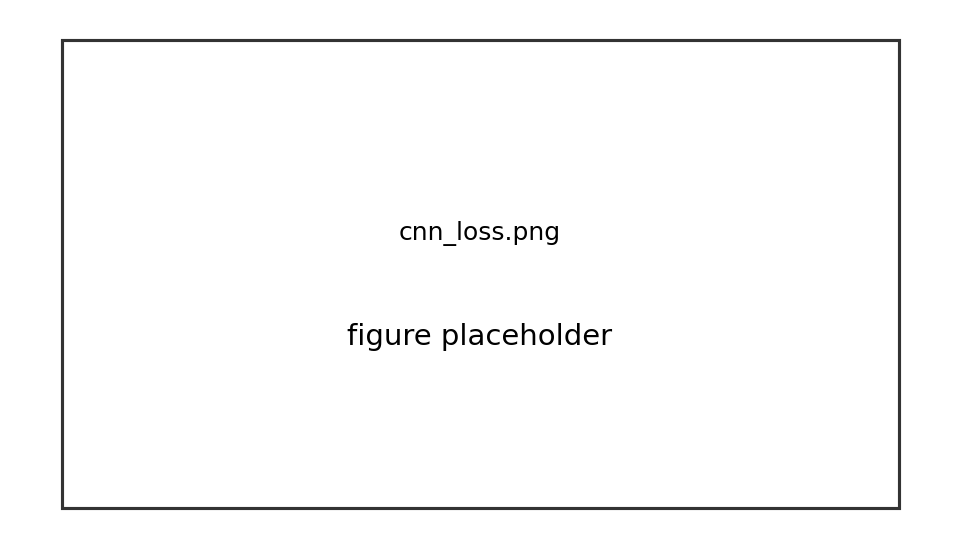
\includegraphics[width=\linewidth,height=0.23\textheight,keepaspectratio]{cnn_loss.png}
    \end{column}
    \begin{column}{0.48\textwidth}\centering
      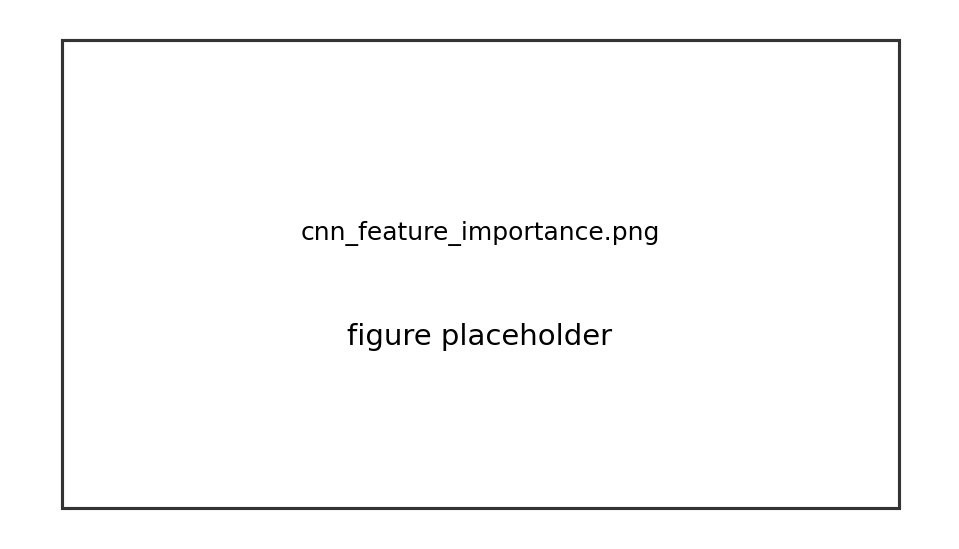
\includegraphics[width=\linewidth,height=0.23\textheight,keepaspectratio]{cnn_feature_importance.png}
    \end{column}
  \end{columns}
  \source{训练损失继续下降而验证损失回升，说明容量控制与早停不可省略。}
\end{frame}

% 31
\begin{frame}{备份｜组合、换手与成本如何计算？}
  \begin{columns}[T,onlytextwidth]
    \begin{column}{0.48\textwidth}
      \begin{block}{组合形成}
        每5个交易日按预测排序；至少8个有效品种；做多最高20\%、做空最低20\%；两侧绝对权重各0.5，组内等权。
      \end{block}
      \begin{equation*}
        \mathrm{TO}_t=\sum_i|w_{i,t}-w_{i,t^-}|
      \end{equation*}
    \end{column}
    \begin{column}{0.48\textwidth}
      \begin{block}{成本后收益}
        \begin{equation*}
          r^{net}_{p,t}=\sum_i w_{i,t}y^{(5)}_{i,t}-\mathrm{TO}_t\frac{c}{10,000}
        \end{equation*}
        $c\in\{0,3,5,10\}$bps；主口径5bps；按$252/5=50.4$期年化。
      \end{block}
      \begin{alertblock}{尚未完整计入}
        统一的精确涨跌停延迟成交与换月额外冲击成本。
      \end{alertblock}
    \end{column}
  \end{columns}
\end{frame}

% 32
\begin{frame}{备份｜完整模型成本敏感性}
  \begin{columns}[T,onlytextwidth]
    \begin{column}{0.55\textwidth}
      \small
      \begin{tabular}{lrrrr}
        \toprule
        模型年化收益 & 0bps & 3bps & 5bps & 10bps \\
        \midrule
        HCGNN持续 & 4.05\% & 3.49\% & 3.11\% & 2.18\% \\
        Conv--Transformer & 2.62\% & 1.73\% & 1.14\% & -0.32\% \\
        \bottomrule
      \end{tabular}
      \medskip
      \small 5bps下：Ridge $-1.79\%$；等权 $-1.88\%$；LightGBM $-2.12\%$。
    \end{column}
    \begin{column}{0.41\textwidth}
      \centering
      
\includegraphics[width=\linewidth,height=0.50\textheight,keepaspectratio]{v6_fee_sensitivity.png}
    \end{column}
  \end{columns}
  \vfill
  \begin{takeaway}[成本解释]
    费用曲线变平主要来自换手下降；不能把“更耐成本”全部归因于更深的网络结构。
  \end{takeaway}
\end{frame}

% 33
\begin{frame}{备份｜年度、期限与延迟稳健性}
  \begin{columns}[T,onlytextwidth]
    \begin{column}{0.63\textwidth}
      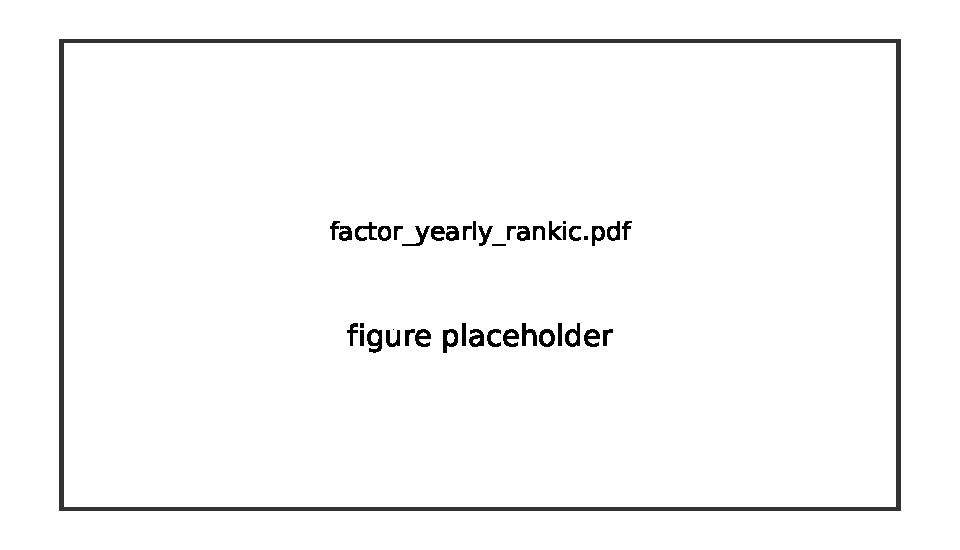
\includegraphics[width=\linewidth,height=0.58\textheight,keepaspectratio]{factor_yearly_rankic.pdf}
    \end{column}
    \begin{column}{0.33\textwidth}
      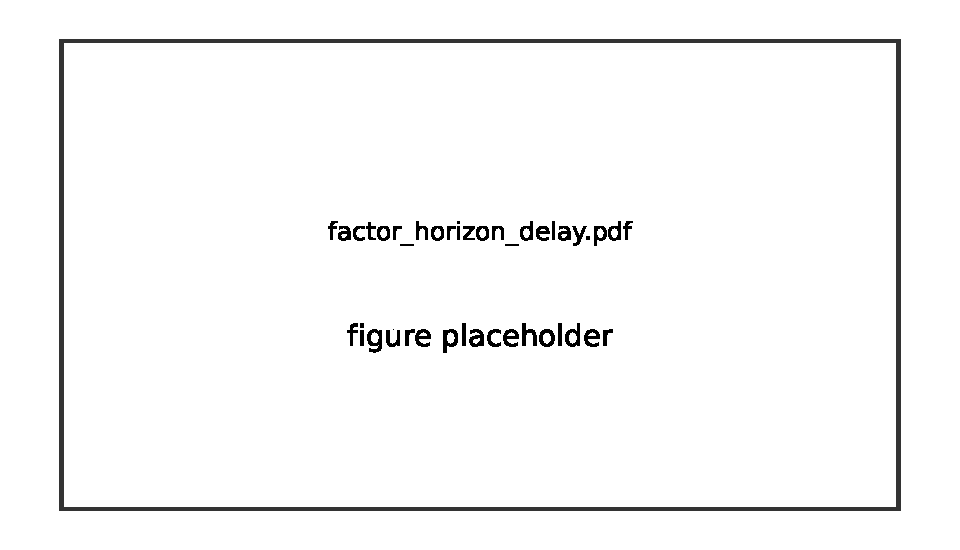
\includegraphics[width=\linewidth,height=0.30\textheight,keepaspectratio]{factor_horizon_delay.pdf}
      \smallskip
      \scriptsize
      预测期限：1/5/20日\par
      趋势邻域：10/20/40或40/60/80日\par
      Conv即时/延迟Rank IC：0.0069/0.0054\par
      20日近似Rank IC：0.0121
    \end{column}
  \end{columns}
\end{frame}

% 34
\begin{frame}{备份｜统计推断与多重检验}
  \centering
  \begin{tikzpicture}[
    node distance=6mm,
    gate/.style={draw=AcademicLine,fill=AcademicWhite,rounded corners=2pt,text width=27mm,minimum height=18mm,align=center,font=\small},
    a/.style={-{Stealth[length=2mm]},draw=AcademicNavy,thick}
  ]
    \node[gate] (g1) {\keyterm{原始效果}\par Rank IC / 收益};
    \node[gate,right=of g1] (g2) {\keyterm{时间依赖}\par 5阶NW/HAC};
    \node[gate,right=of g2] (g3) {\keyterm{多重检验}\par BH--FDR};
    \node[gate,right=of g3] (g4) {\keyterm{经济门槛}\par 5bps净收益};
    \draw[a] (g1)--(g2); \draw[a] (g2)--(g3); \draw[a] (g3)--(g4);
  \end{tikzpicture}
  \vfill
  \begin{columns}[T,onlytextwidth]
    \begin{column}{0.48\textwidth}
      \begin{alertblock}{因子层}
        A类要求FDR $q\le0.10$；最终A类数量为0，即正Rank IC不等于已统计确认。
      \end{alertblock}
    \end{column}
    \begin{column}{0.48\textwidth}
      \begin{alertblock}{模型层}
        Conv 5bps收益HAC $p=0.636$；LightGBM 5bps HAC $p=0.596$。
      \end{alertblock}
    \end{column}
  \end{columns}
\end{frame}

% 35
\begin{frame}{备份｜证据状态与答辩边界}
  \small
  \begin{tabularx}{\textwidth}{@{}p{3.2cm}Xp{3.0cm}@{}}
    \toprule
    \keyterm{项目要素} & \keyterm{当前证据状态} & \keyterm{答辩表述} \\
    \midrule
    92字段 / 2019--2025 / 5日标签 & 已冻结统一接口与时间折 & 可称统一样本外框架 \\
    HCGNN产业关系 & 当前关系定义下得到OOS结果；精确生产配比仍待冻结 & 称“结构化图关系”，不夸大为完整产业链真值 \\
    仓单紧张度Rank IC & 不同汇总表约0.0230/0.0236 & 回到底表统一精度，不回避版本差异 \\
    涨跌停和换月冲击 & 部分代理；额外换月冲击当前为0 & 不称完整实盘模拟 \\
    真实手续费 & 覆盖约73.16\%，早期较弱 & 报告主口径仍为统一5bps \\
    \bottomrule
  \end{tabularx}
  \vfill
  \begin{takeaway}[最终答辩纪律]
    不说“显著提高收益”、不说“发现8个有效Alpha”、不说“完整模拟实盘”；只陈述统一协议下证据实际支持的结论。
  \end{takeaway}
\end{frame}

\end{document}
